\section{Smart Pixels for LHC}
{{\footnotesize
\begin{description}[labelwidth=5em, labelsep=1em, leftmargin=*, align=left, itemsep=0.3em, parsep=0em]
  \item[date:] 2024-06-24
  \item[version:] TODO
  \item[last\_updated:] 2024-06
  \item[expired:] unknown
  \item[valid:] yes
  \item[valid\_date:] TODO
  \item[url:] \href{https://arxiv.org/abs/2406.14860}{https://arxiv.org/abs/2406.14860}
  \item[doi:] TODO
  \item[domain:] Particle Physics; Instrumentation and Detectors
  \item[focus:] On-sensor, in-pixel ML filtering for high-rate LHC pixel detectors
  \item[keywords:]
    - smart pixel
    - on-sensor inference
    - data reduction
    - trigger
  \item[summary:] Presents a 256x256-pixel ROIC in 28 nm CMOS with embedded 2-layer NN for cluster filtering
at 25 ns, achieving 54-75\% data reduction while maintaining noise and latency constraints. Prototype
consumes \textasciitilde{}300 microW/pixel and operates in combinatorial digital logic.

  \item[licensing:] TODO
  \item[task\_types:]
    - Image Classification
    - Data filtering
  \item[ai\_capability\_measured:]
    - On-chip
    - low-power inference; data reduction
  \item[metrics:]
    - Data rejection rate
    - Power per pixel
  \item[models:]
    - 2-layer pixel NN
  \item[ml\_motif:]
    - Real-time, Image/CV
  \item[type:] Benchmark
  \item[ml\_task:]
    - Image Classification
  \item[solutions:] TODO
  \item[notes:] Prototype in CMOS 28 nm; proof-of-concept for Phase III pixel upgrades.

  \item[contact.name:] Lindsey Gray; Jennet Dickinson
  \item[contact.email:] unknown
  \item[results.links.name:] ChatGPT LLM
  \item[fair.reproducible:] True
  \item[fair.benchmark\_ready:] Yes (Zenodo:7331128)
  \item[ratings.software.rating:] 0
  \item[ratings.software.reason:] Not analyzed. 

  \item[ratings.specification.rating:] 9.0
  \item[ratings.specification.reason:] Task (automated neural architecture search for real-time physics) is well formulated with clear latency, model compression, and deployment goals.

  \item[ratings.dataset.rating:] 6.0
  \item[ratings.dataset.reason:] Internal Bragg and jet datasets used; not publicly hosted or FAIR-compliant, though mentioned in the paper.

  \item[ratings.metrics.rating:] 10.0
  \item[ratings.metrics.reason:] BOP reduction, latency, and accuracy are all quantitatively evaluated.

  \item[ratings.reference\_solution.rating:] 8.0
  \item[ratings.reference\_solution.reason:] NAC-generated models for Bragg peak and jet classification are described, but pipeline requires integration of several tools and is not fully packaged.

  \item[ratings.documentation.rating:] 7.0
  \item[ratings.documentation.reason:] NAC pipeline, hls4ml usage, and results are discussed; code (e.g., nac-opt) referenced, but replication requires stitching together toolchain and data.

  \item[id:] smart\_pixels\_for\_lhc
  \item[Citations:] \cite{parpillon2024smartpixelsinpixelai}
  \item[Ratings:]
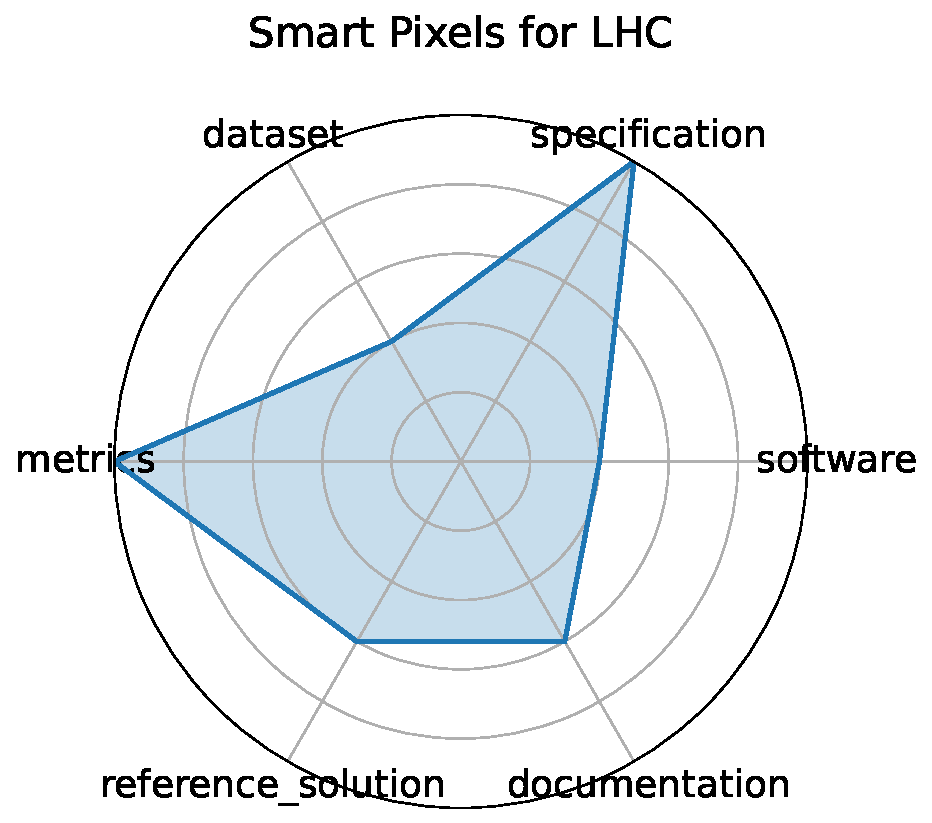
\includegraphics[width=0.2\textwidth]{smart_pixels_for_lhc_radar.pdf}
\end{description}
}}
\clearpage